\section[Modellazione di un dataset di bike sharing]{Modellazione di un dataset di bike sharing}
\begin{frame}
	\frametitle{Descrizione del dataset}
	
	Il dataset inerente il bike sharing è così composto:
	\begin{itemize}
		\justifying
		\item \textbf{variabile dipendente}: l'oggetto del caso di studio consiste nel numero di ritiri orari di biciclette presso le stazioni della rete di bike sharing;
		\item \textbf{variabili meteorologiche}: covariate spazio-invarianti come temperatura percepita, piovosità, visibilità orizzontale, velocità del vento e copertura nuvolosa;
		\item \textbf{variabili spaziali}: covariate tempo-invarianti quali la distanza dalla stazione ferroviaria più vicina e la densità demografica nella zona circostante;
		\item \textbf{variabili dummy}: eventi come il lockdown COVID-\num{19}, il ritorno alla vita quotidiana post-lockdown, i weekend e le festività federali sono modellati come variabili categoriche binarie.
	\end{itemize}	
\end{frame}

\begin{frame}
	\centering
	\begin{columns}[T]
		\begin{column}[t]{0.48\linewidth}
			\centering
			\begin{figure}
				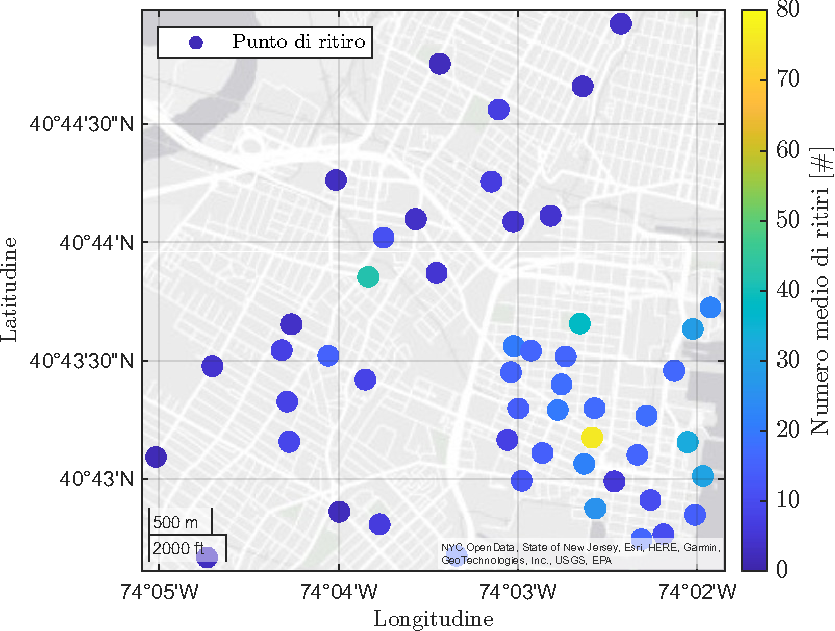
\includegraphics[width=\textwidth]{../Tesi/Immagini/4. Caso di studio/Mappe/Mappa ritiri, inverno}
			\end{figure}
		\end{column}
		\begin{column}[t]{0.48\linewidth}
			\centering
			\begin{figure}
				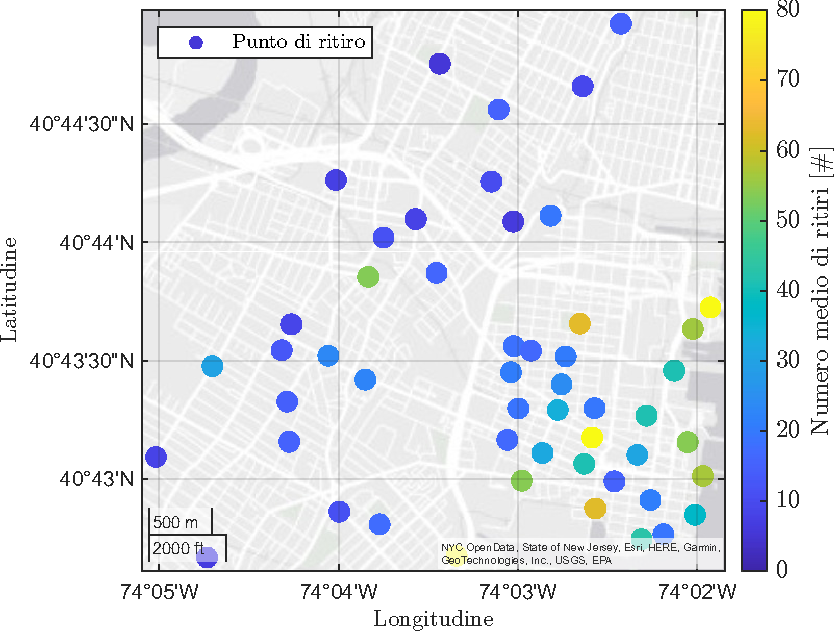
\includegraphics[width=\textwidth]{../Tesi/Immagini/4. Caso di studio/Mappe/Mappa ritiri, estate}
			\end{figure}
		\end{column}
	\end{columns}
	\vspace{5pt}
	\textit{Distribuzione spaziale del numero medio di ritiri giornaliero presso i 51 punti di ritiro, in inverno (sinistra) e in estate (destra)}.
\end{frame}

\begin{frame}
	\centering
	\begin{columns}[T]
		\begin{column}[t]{0.48\linewidth}
			\centering
			\begin{figure}
				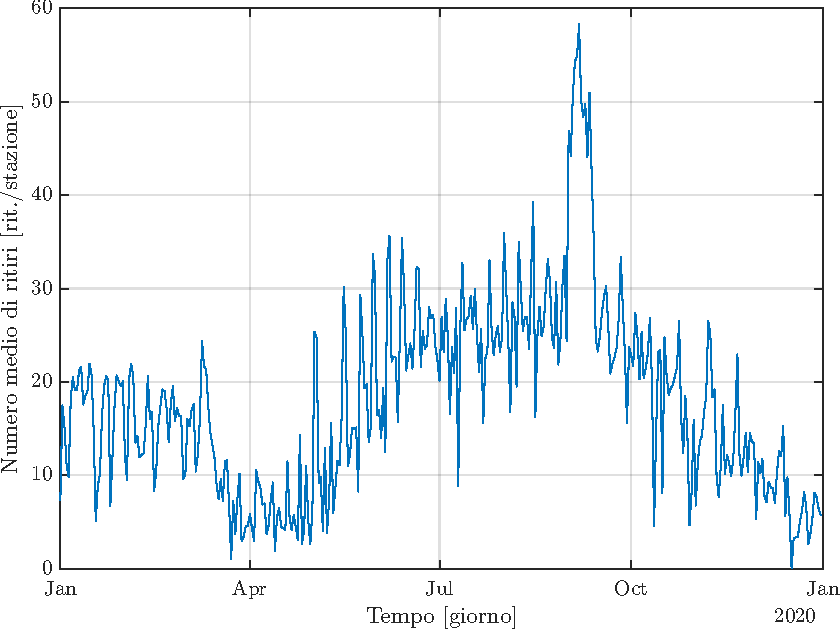
\includegraphics[width=\textwidth]{../Tesi/Immagini/4. Caso di studio/Serie storiche/Ritiri giornalieri}
			\end{figure}
		\end{column}
		\begin{column}[t]{0.48\linewidth}
			\centering
			\begin{figure}
				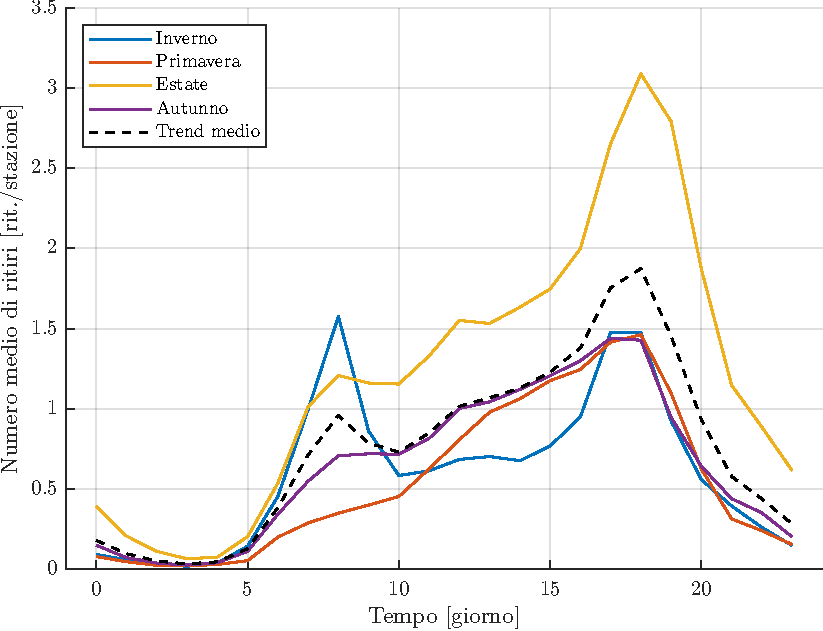
\includegraphics[width=\textwidth]{../Tesi/Immagini/4. Caso di studio/Serie storiche/Ritiri orari}
			\end{figure}
		\end{column}
	\end{columns}
	\vspace{5pt}
	\textit{Andamento giornaliero (sinistra) e orario (destra) del numero medio di ritiri al variare della stagione.}
\end{frame}

\begin{frame}
	\centering
			\begin{figure}
				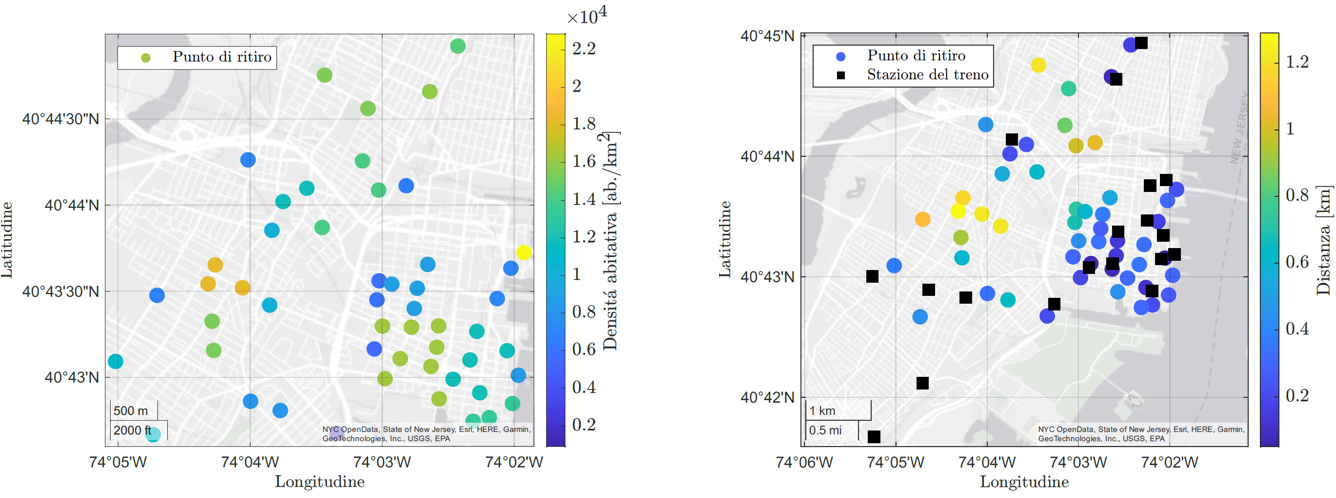
\includegraphics[width=\textwidth]{../Tesi/Immagini/4. Caso di studio/Mappe/Mappa punti ritiro e stazioni treno e densita ab AGGREGATA}
			\end{figure}
	\vspace{-5px}
	\textit{Mappe della densità abitativa nei pressi dei punti di ritiro (sinistra) e delle distanze dei punti di interscambio dalla stazione ferroviaria più vicina (destra).}
\end{frame}

\begin{frame}
	\frametitle{Metodologia}
	\centering
	\begin{enumerate}
		\justifying
		\item \textbf{Cross-validazione con $k=5$ per determinare il valore del parametro $\rho$}: al fine di determinare il $\rho$ ottimale, come metrica è stato impiegato il MSE:
		\begin{equation*}
			MSE = \frac{1}{P}\sum_{i=1}^{k=5}\frac{1}{\text{card}(\mathcal{S}_{val})_i}\sum_{\mathbf{s}\in\mathcal{S}_{val}}^{}\sum_{t=1}^{T}\sum_{l\in\mathcal{L}}^{} (y(\mathbf{s}, l, t) - \hat{y}(\mathbf{s}, l, t))^2
		\end{equation*}
		\begin{equation*}
			P = k\cdot T\cdot q
		\end{equation*}
		\item \textbf{Scelta delle covariate più significative (model selection)}: l'obiettivo è visualizzare le spline per i parametri $\boldsymbol{\beta}$ e i relativi intervalli di confidenza al fine di escludere i regressori poco significativi.

	\end{enumerate}	
\end{frame}
\begin{frame}
	\centering
	
	\begin{enumerate}
		\setcounter{enumi}{2}
		\justifying
		\item \textbf{Validazione del modello finale tramite LOOCV}: per valutare la bontà complessiva del modello definitivo, è stato utilizzato il RMSE:
		\begin{equation*}
			RMSE_\mathbf{s} = \sqrt{\frac{1}{T\cdot q}\sum_{t=1}^{T}\sum_{l\in\mathcal{L}}^{} (y(\mathbf{s}, l, t) - \hat{y}(\mathbf{s}, l, t))^2}
		\end{equation*}
		\item \textbf{Previsione spaziale utilizzando il kriging}: è stato stimato il volume di noleggi orario così definito:
		\begin{equation*}
			v(\mathbf{s}, l|\mathcal{T}) = \sum_{t\in\mathcal{T}} \hat{y}(\mathbf{s}, l, t), \ \forall \mathbf{s}\in\mathcal{D}, \ \forall l\in\mathcal{H}, \mathcal{T} = 152,\dots,213
		\end{equation*}
			Dopodiché, i \num{24} valori di $v(\mathbf{s}, l|\mathcal{T})$ sono stati così raggruppati:
		\begin{equation*}
			\bar{v}(\mathbf{s}, l|\mathcal{T})_i = \frac{1}{\text{card}(\mathcal{R}_i)}\sum_{j\in\mathcal{R}_i}^{}v(\mathbf{s}, j|\mathcal{T}), \ i=1,\dots, 6
		\end{equation*}
	\end{enumerate}	
\end{frame}

\begin{frame}
	\frametitle{Cross-validazione per determinare il valore di $\rho$}
	\centering
	\begin{figure}
		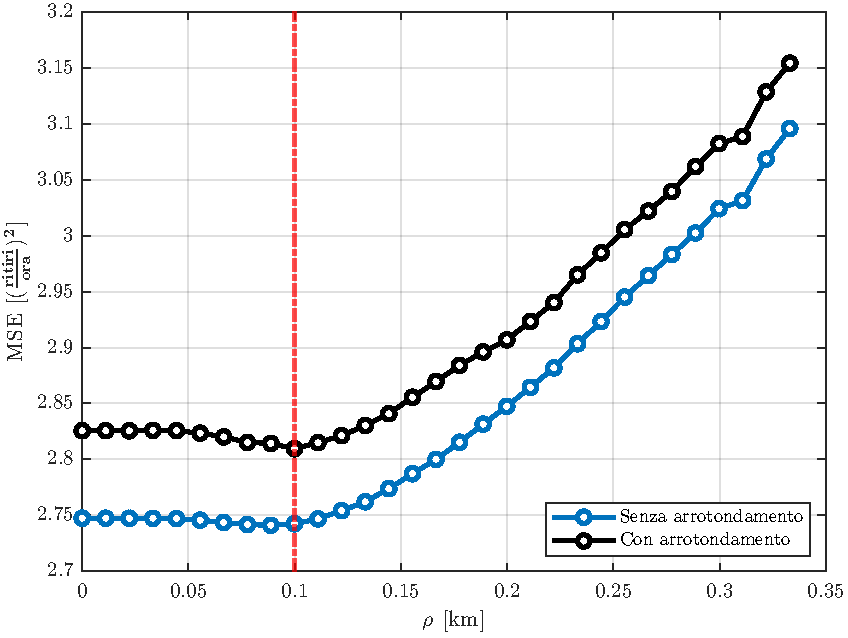
\includegraphics[height=130px]{../Tesi/Immagini/4. Caso di studio/Cross_validazione/MSE_rho_full_focus}
	\end{figure}
	\vspace{-10pt}
	\textit{Andamento del $MSE$ in cross-validazione con e senza arrotondamento al variare del parametro $\rho$.}
\end{frame}

\begin{frame}
	\frametitle{Model selection}
	\centering
	\begin{figure}
		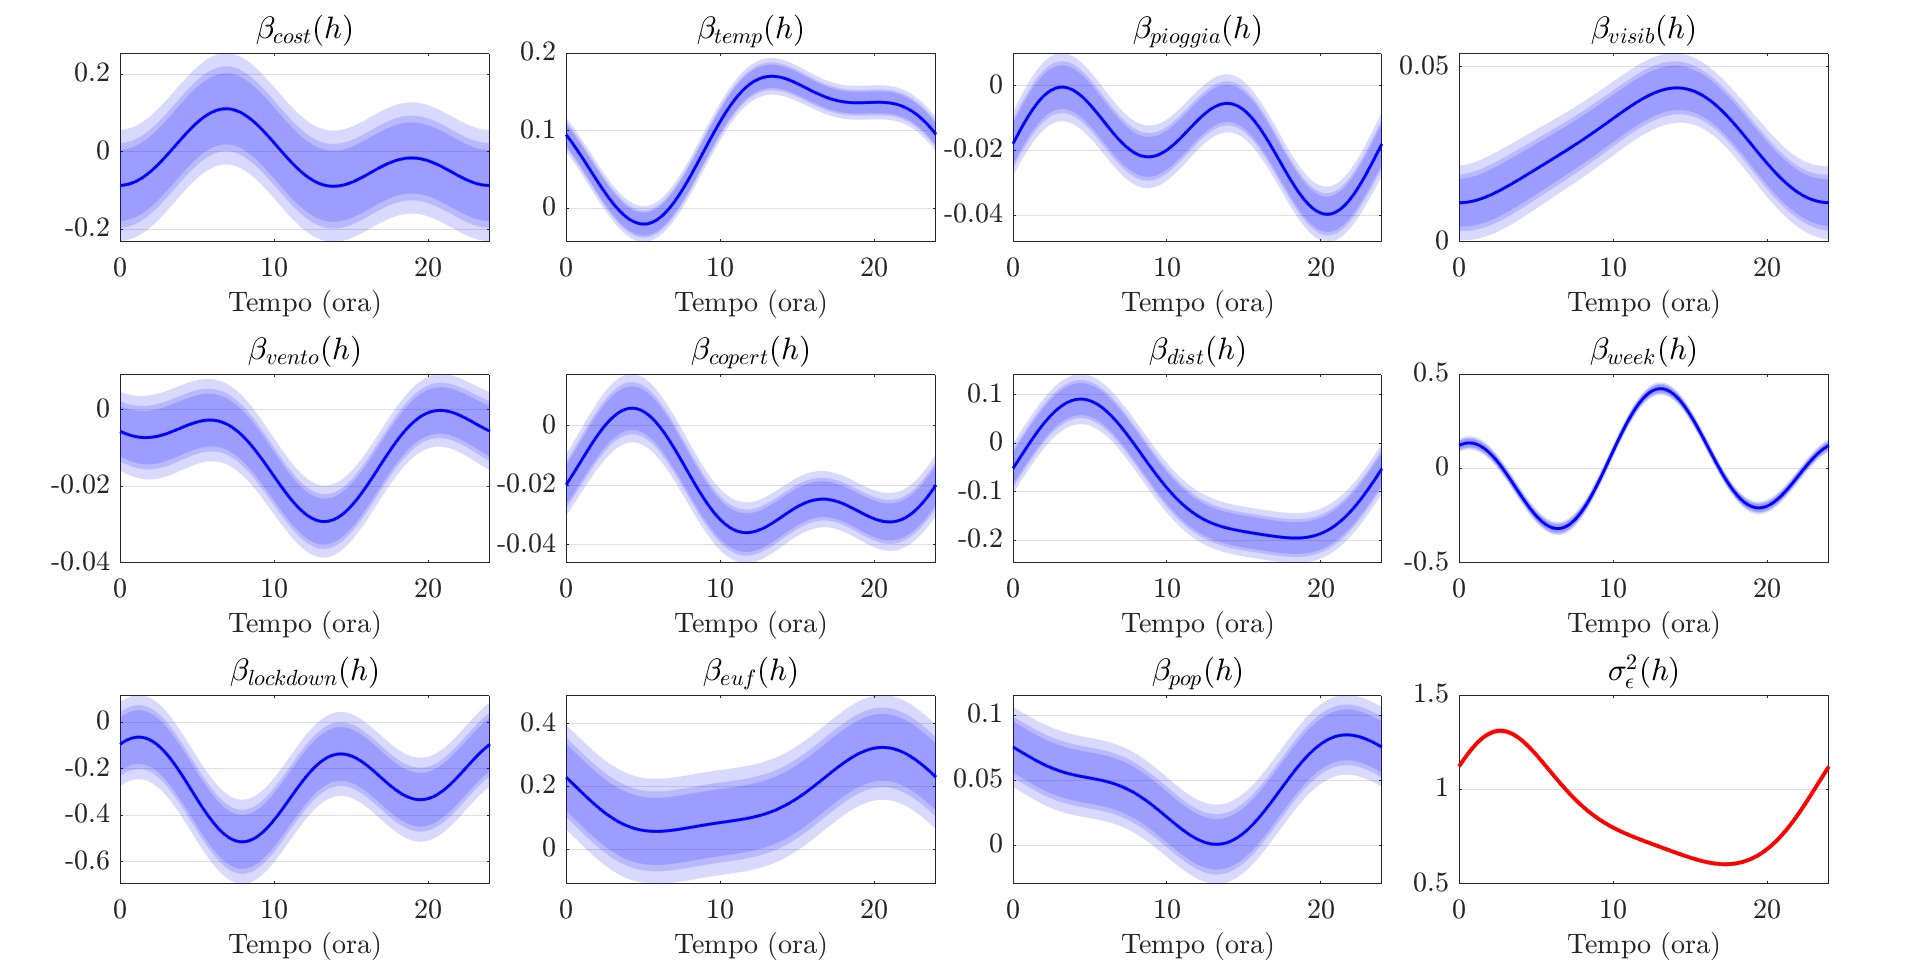
\includegraphics[height=140px]{../Tesi/Immagini/4. Caso di studio/Model selection/Trend spline, rho=100m}
	\end{figure}
	\vspace{-10pt}
	\textit{Spline di Fourier per i coefficienti $\boldsymbol{\beta}$ e rispettivi intervalli di confidenza}
\end{frame}

\begin{frame}
	\frametitle{Validazione del modello definitivo}
	\centering
	
	\begin{figure}
		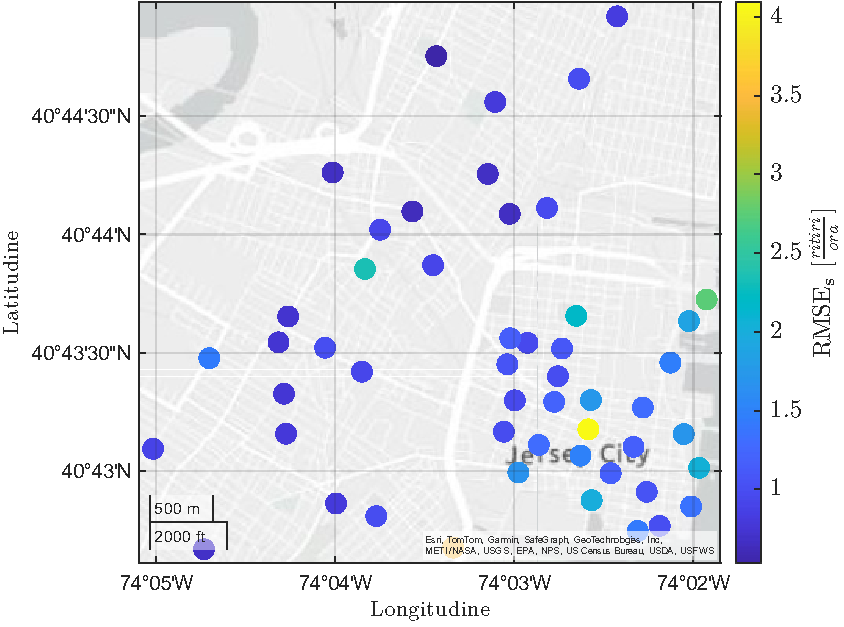
\includegraphics[height=140px]{../Tesi/Immagini/4. Caso di studio/LOOCV/RMSE_s}
	\end{figure}
	\vspace{-10pt}
	\textit{Mappa della distribuzione del $RMSE_\mathbf{s}$}
\end{frame}

\begin{frame}
	\frametitle{Previsione spaziale tramite Kriging}
	\centering
	
	\begin{columns}
		\begin{column}{0.33\linewidth}
			\centering
			\begin{figure}
				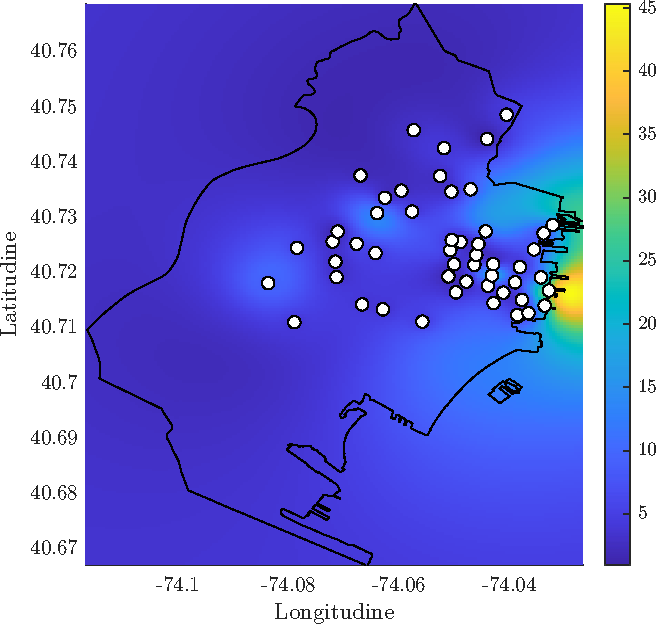
\includegraphics[width=\textwidth]{../Tesi/Immagini/4. Caso di studio/Kriging/Mappa volume, 1}
			\end{figure}
		\end{column}
		\begin{column}{0.33\linewidth}
			\centering
			\begin{figure}
				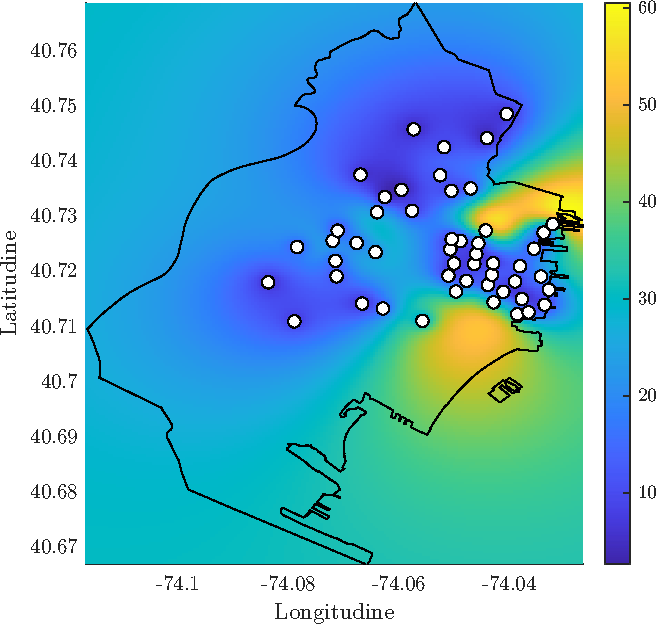
\includegraphics[width=\textwidth]{../Tesi/Immagini/4. Caso di studio/Kriging/Mappa volume, 2}
			\end{figure}
		\end{column}
		\begin{column}{0.33\linewidth}
			\centering
			\begin{figure}
				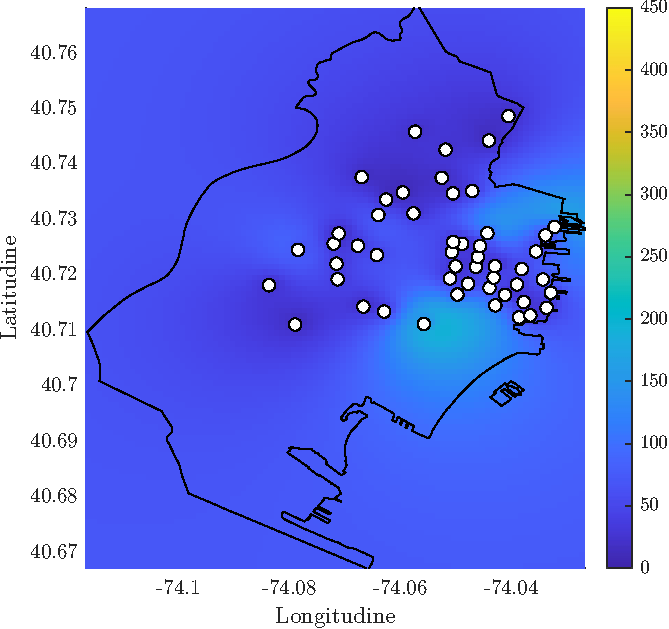
\includegraphics[width=\textwidth]{../Tesi/Immagini/4. Caso di studio/Kriging/Mappa volume, 3}
			\end{figure}
		\end{column}
	\end{columns}
	\vspace{10pt}
	\textit{Volume del numero di ritiri previsti, raggruppati per fasce orarie: dalle 00:01 alle 04:00 (sinistra), dalle 04:01 alle 08:00 (centro), dalle 08:01 alle 12:00 (destra).}
\end{frame}

\begin{frame}
	\centering
	\begin{columns}
		\begin{column}{0.33\linewidth}
			\centering
			\begin{figure}
				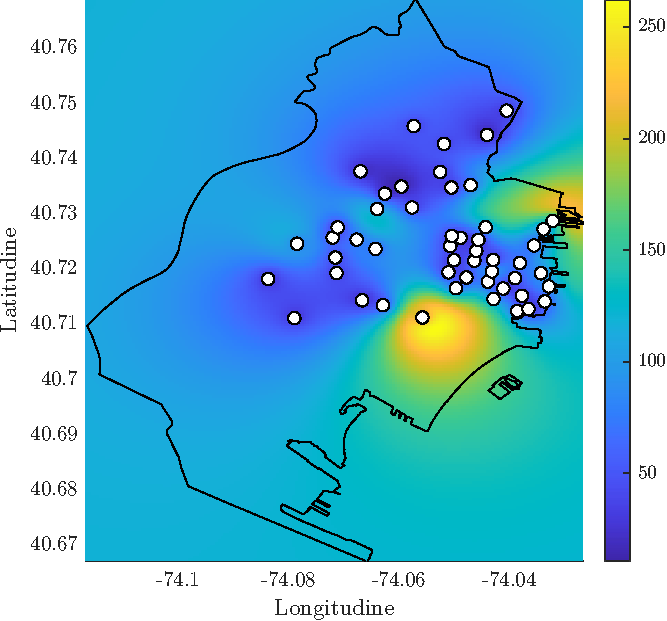
\includegraphics[width=\textwidth]{../Tesi/Immagini/4. Caso di studio/Kriging/Mappa volume, 4}
			\end{figure}
		\end{column}
		\begin{column}{0.33\linewidth}
			\centering
			\begin{figure}
				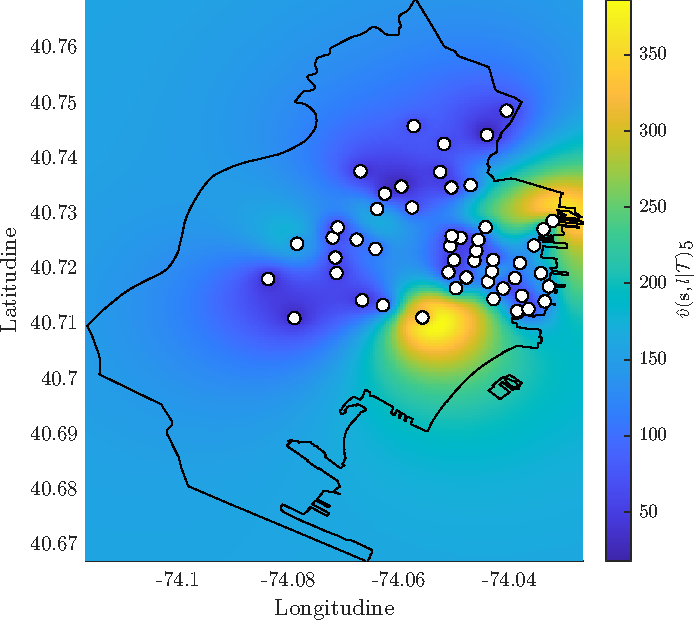
\includegraphics[width=\textwidth]{../Tesi/Immagini/4. Caso di studio/Kriging/Mappa volume, 5}
			\end{figure}
		\end{column}
		\begin{column}{0.33\linewidth}
			\centering
			\begin{figure}
				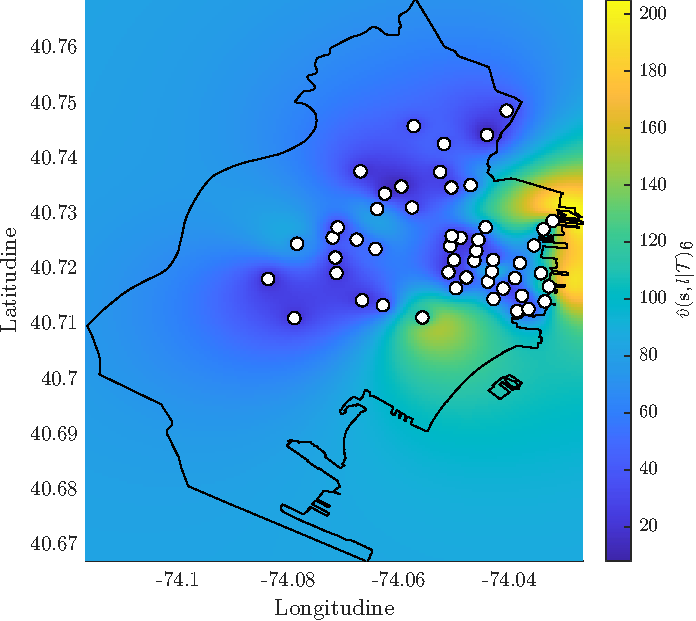
\includegraphics[width=\textwidth]{../Tesi/Immagini/4. Caso di studio/Kriging/Mappa volume, 6}
			\end{figure}
		\end{column}
	\end{columns}
	\vspace{10pt}
	\textit{Volume del numero di ritiri previsti, raggruppati per fasce orarie: dalle 12:01 alle 16:00 (sinistra), dalle 16:01 alle 20:00 (centro), dalle 20:01 alle 24:00 (destra).}
\end{frame}